\subsection{UC5 - Creazione riunione su piattaforma esterna}
\begin{itemize}
    \item \textbf{Identificativo}: UC5
    \item \textbf{Nome}: Creazione riunione su piattaforma esterna
    \item \textbf{Descrizione grafica}:
\end{itemize}

\begin{figure}[h]
   \centering
   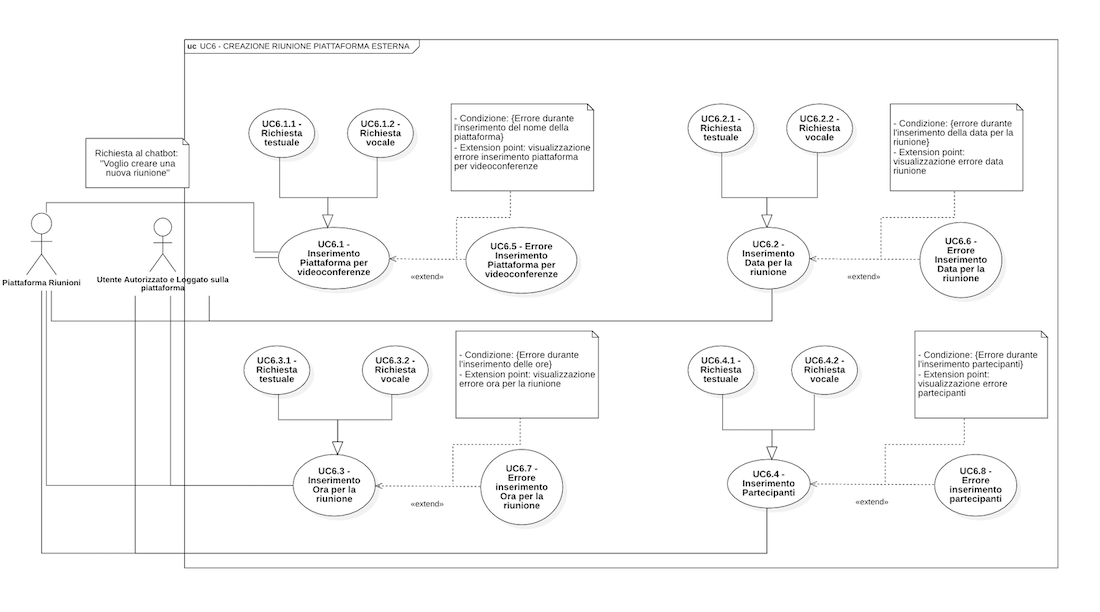
\includegraphics[scale=0.9]{images/UC5.png} 
   \caption{Descrizione grafica caso d'uso UC5}
\end{figure}

 \begin{itemize}
    \item \textbf{Attori}
 \begin{itemize} 
    \item \textit{Primari}: utente autorizzato e loggato sulla piattaforma per videoconferenze
    \item \textit{Secondari}: non presenti
 \end{itemize}
 \item \textbf{Precondizione}: l'utente è autorizzato e loggato sulla piattaforma esterna per videoconferenze desiderata, e si trova nell'interfaccia del chatbot.
 \item \textbf{Postcondizione}: il chatbot risponde alla richiesta dell'utente e invia la richiesta per la creazione della riunione.
 \item \textbf{Scenario principale}: l'utente autorizzato e loggato sulla piattaforma per videoconferenze richiede la creazione di una riunione, specificando la piattaforma (UC5.1), la data (UC5.2) e l'ora (UC5.3) desiderati e la lista dei partecipanti (UC5.4).
 \item \textbf{Estensioni}: 
 \begin{itemize} 
    \item il chatbot comunica all'utente che uno o più parametri specificati non sono corretti (UC5.5 UC5.6 UC5.7 UC5.8).
 \end{itemize}
\end{itemize}
\newpage

\subsubsection{UC5.1 - Inserimento piattaforma per videoconferenze}
\begin{itemize}
    \item \textbf{Identificativo}: UC5.1
    \item \textbf{Nome}: inserimento piattaforma per videoconferenze
    \item \textbf{Descrizione grafica}: (approfondita in UC5)
    \item \textbf{Attori}
 \begin{itemize} 
    \item \textit{Primari}: utente autorizzato e loggato sulla piattaforma per videoconferenze
    \item \textit{Secondari}: non presenti
 \end{itemize}
 \item \textbf{Precondizione}: l'utente comunica al chatbot la richiesta di creazione di una riunione.
 \item \textbf{Postcondizione}: l'utente ha comunicato al chatbot la piattaforma sulla quale verrà creata la riunione.
 \item \textbf{Scenario principale}: il chatbot chiede all'utente su quale applicazione desidera creare la riunione. L'utente comunica al chatbot la piattaforma tramite messaggio testuale (UC5.1.1) o vocale (UC5.1.2).
 \item \textbf{Estensioni}: 
 \begin{itemize} 
    \item il chatbot comunica all'utente che la piattaforma per videoconferenze inserita non è corretta (UC5.5).
 \end{itemize}
\end{itemize}

\paragraph{UC5.1.1 - Richiesta Testuale}
\begin{itemize}
   \item \textbf{Identificativo}: UC5.1.1
   \item \textbf{Nome}: Richiesta testuale
   \item \textbf{Descrizione grafica}: (approfondita in UC5)
   \item \textbf{Attori}:
   \begin{itemize} 
       \item \textit{Primari}: utente autorizzato
       \item \textit{Secondari}: non presenti
   \end{itemize}
       \item \textbf{Precondizione}: l'utente si è autenticato al sistema e ha richiesto di voler creare una riunione su una piattaforma esterna.
       \item \textbf{Postcondizione}: l'utente fornisce il nome della piattaforma di videoconferenze, su cui voler creare la riunione.
    \item \textbf{Scenario principale}: 
       \begin{itemize}
           \item L'utente ha effettuato l'accesso al sistema 
           \item L'utente fornisce tramite input testuale il nome della piattaforma, su cui vuole creare la riunione
       \end{itemize}
\end{itemize}

\paragraph{UC5.1.2 - Richiesta Vocale}
\begin{itemize}
   \item \textbf{Identificativo}: UC5.1.2
   \item \textbf{Nome}: Richiesta vocale
   \item \textbf{Descrizione grafica}: (approfondita in UC5)
   \item \textbf{Attori}:
   \begin{itemize} 
       \item \textit{Primari}: utente autorizzato
       \item \textit{Secondari}: non presenti
   \end{itemize}
       \item \textbf{Precondizione}: l'utente si è autenticato al sistema e ha richiesto di voler creare una riunione su una piattaforma esterna.
       \item \textbf{Postcondizione}: l'utente fornisce il nome della piattaforma di videoconferenze, su cui voler creare la riunione.
    \item \textbf{Scenario principale}: 
       \begin{itemize}
           \item L'utente ha effettuato l'accesso al sistema 
           \item L'utente fornisce tramite input vocale il nome della piattaforma, su cui vuole creare la riunione
       \end{itemize}
\end{itemize}

\subsubsection{UC5.2 - Inserimento data per la riunione}
\begin{itemize}
    \item \textbf{Identificativo}: UC5.2
    \item \textbf{Nome}: inserimento data per la riunione
    \item \textbf{Descrizione grafica}: (approfondita in UC5)
    \item \textbf{Attori}
 \begin{itemize} 
    \item \textit{Primari}: utente autorizzato e loggato sulla piattaforma per videoconferenze
    \item \textit{Secondari}: non presenti
 \end{itemize}
 \item \textbf{Precondizione}: l'utente comunica al chatbot la richiesta di creazione di una riunione.
 \item \textbf{Postcondizione}: l'utente ha comunicato al chatbot la data alla quale verrà creata la riunione.
 \item \textbf{Scenario principale}: il chatbot chiede all'utente in che data desidera creare la riunione. L'utente comunica al chatbot la data tramite messaggio testuale (UC5.1.1) o vocale (UC5.1.2).
 \item \textbf{Estensioni}: 
 \begin{itemize} 
    \item il chatbot comunica all'utente che la data inserita non è corretta, oppure risulta indisponibile (UC5.6).
 \end{itemize}
\end{itemize}

\paragraph{UC5.2.1 - Richiesta Testuale}
\begin{itemize}
   \item \textbf{Identificativo}: UC5.2.1
   \item \textbf{Nome}: Richiesta testuale
   \item \textbf{Descrizione grafica}: (approfondita in UC5)
   \item \textbf{Attori}:
   \begin{itemize} 
       \item \textit{Primari}: utente autorizzato
       \item \textit{Secondari}: non presenti
   \end{itemize}
       \item \textbf{Precondizione}: l'utente si è autenticato al sistema e ha richiesto di voler creare una riunione su una piattaforma esterna.
       \item \textbf{Postcondizione}: l'utente fornisce la data per quando voler creare la riunione.
    \item \textbf{Scenario principale}: 
       \begin{itemize}
           \item L'utente ha effettuato l'accesso al sistema 
           \item L'utente fornisce tramite input testuale la data in cui avverrà la riunione
       \end{itemize}
\end{itemize}

\paragraph{UC5.2.2- Richiesta Vocale}
\begin{itemize}
   \item \textbf{Identificativo}: UC5.2.2
   \item \textbf{Nome}: Richiesta vocale
   \item \textbf{Descrizione grafica}: (approfondita in UC5)
   \item \textbf{Attori}:
   \begin{itemize} 
       \item \textit{Primari}: utente autorizzato
       \item \textit{Secondari}: non presenti
   \end{itemize}
       \item \textbf{Precondizione}: l'utente si è autenticato al sistema e ha richiesto di voler creare una riunione su una piattaforma esterna.
       \item \textbf{Postcondizione}: l'utente fornisce la data per quando voler creare la riunione.
    \item \textbf{Scenario principale}: 
       \begin{itemize}
           \item L'utente ha effettuato l'accesso al sistema 
           \item L'utente fornisce tramite input vocale la data in cui avverrà la riunione
       \end{itemize}
\end{itemize}

\subsubsection{UC5.3 - Inserimento ora per la riunione}
\begin{itemize}
    \item \textbf{Identificativo}: UC5.3
    \item \textbf{Nome}: inserimento ora per la riunione
    \item \textbf{Descrizione grafica}: (approfondita in UC5)
    \item \textbf{Attori}
 \begin{itemize} 
    \item \textit{Primari}: utente autorizzato e loggato sulla piattaforma per videoconferenze
    \item \textit{Secondari}: non presenti
 \end{itemize}
 \item \textbf{Precondizione}: l'utente comunica al chatbot la richiesta di creazione di una riunione.
 \item \textbf{Postcondizione}: l'utente ha comunicato al chatbot l'ora alla quale verrà creata la riunione.
 \item \textbf{Scenario principale}: il chatbot chiede all'utente a che ora desidera creare la riunione. L'utente comunica al chatbot l'ora tramite messaggio testuale (UC5.1.1) o vocale (UC5.1.2).
 \item \textbf{Estensioni}: 
 \begin{itemize} 
    \item il chatbot comunica all'utente che l'ora inserita non è corretta, oppure risulta indisponibile (UC5.7).
 \end{itemize}
\end{itemize}

\paragraph{UC5.3.1 - Richiesta Testuale}
\begin{itemize}
   \item \textbf{Identificativo}: UC5.3.1
   \item \textbf{Nome}: Richiesta testuale
   \item \textbf{Descrizione grafica}: (approfondita in UC5)
   \item \textbf{Attori}:
   \begin{itemize} 
       \item \textit{Primari}: utente autorizzato
       \item \textit{Secondari}: non presenti
   \end{itemize}
       \item \textbf{Precondizione}: l'utente si è autenticato al sistema e ha richiesto di voler creare una riunione su una piattaforma esterna.
       \item \textbf{Postcondizione}: l'utente fornisce l'ora alla quale avverrà la riunione.
    \item \textbf{Scenario principale}: 
       \begin{itemize}
           \item L'utente ha effettuato l'accesso al sistema 
           \item L'utente fornisce tramite input testuale l'ora in cui avverrà la riunione
       \end{itemize}
\end{itemize}

\paragraph{UC5.3.2 - Richiesta Vocale}
\begin{itemize}
   \item \textbf{Identificativo}: UC5.3.2
   \item \textbf{Nome}: Richiesta vocale
   \item \textbf{Descrizione grafica}: (approfondita in UC5)
   \item \textbf{Attori}:
   \begin{itemize} 
       \item \textit{Primari}: utente autorizzato
       \item \textit{Secondari}: non presenti
   \end{itemize}
       \item \textbf{Precondizione}: l'utente si è autenticato al sistema e ha richiesto di voler creare una riunione su una piattaforma esterna.
       \item \textbf{Postcondizione}: l'utente fornisce l'ora alla quale avverrà la riunione.
    \item \textbf{Scenario principale}: 
       \begin{itemize}
           \item L'utente ha effettuato l'accesso al sistema 
           \item L'utente fornisce tramite input vocale l'ora in cui avverrà la riunione
       \end{itemize}
\end{itemize}


\subsubsection{UC5.4 - Inserimento partecipanti}
\begin{itemize}
    \item \textbf{Identificativo}: UC5.4
    \item \textbf{Nome}: inserimento partecipanti
    \item \textbf{Descrizione grafica}: (approfondita in UC5)
    \item \textbf{Attori}
 \begin{itemize} 
    \item \textit{Primari}: utente autorizzato e loggato sulla piattaforma per videoconferenze
    \item \textit{Secondari}: non presenti
 \end{itemize}
 \item \textbf{Precondizione}: l'utente comunica al chatbot la richiesta di creazione di una riunione.
 \item \textbf{Postcondizione}: l'utente ha comunicato al chatbot i partecipanti alla riunione che verrà creata.
 \item \textbf{Scenario principale}: il chatbot chiede all'utente quali sono i partecipanti alla riunione. L'utente comunica al chatbot i partecipanti tramite messaggio testuale (UC5.1.1) o vocale (UC5.1.2).
 \item \textbf{Estensioni}: 
 \begin{itemize} 
    \item il chatbot comunica all'utente che uno o più partecipanti non sono stati inseriti in modo corretto (UC5.8).
 \end{itemize}
\end{itemize}

\paragraph{UC5.4.1 - Richiesta Testuale}
\begin{itemize}
   \item \textbf{Identificativo}: UC5.4.1
   \item \textbf{Nome}: Richiesta testuale
   \item \textbf{Descrizione grafica}: (approfondita in UC5)
   \item \textbf{Attori}:
   \begin{itemize} 
       \item \textit{Primari}: utente autorizzato
       \item \textit{Secondari}: non presenti
   \end{itemize}
       \item \textbf{Precondizione}: l'utente si è autenticato al sistema e ha richiesto di voler creare una riunione su una piattaforma esterna.
       \item \textbf{Postcondizione}: l'utente fornisce il nome dei partecipanti in maniera testuale
    \item \textbf{Scenario principale}: 
       \begin{itemize}
           \item L'utente ha effettuato l'accesso al sistema 
           \item L'utente fornisce tramite input testuale il nome dei partecipanti alla riunione
       \end{itemize}
\end{itemize}

\paragraph{UC5.4.2 - Richiesta Vocale}
\begin{itemize}
   \item \textbf{Identificativo}: UC5.4.2
   \item \textbf{Nome}: Richiesta vocale
   \item \textbf{Descrizione grafica}: (approfondita in UC5)
   \item \textbf{Attori}:
   \begin{itemize} 
       \item \textit{Primari}: utente autorizzato
       \item \textit{Secondari}: non presenti
   \end{itemize}
       \item \textbf{Precondizione}: l'utente si è autenticato al sistema e ha richiesto di voler creare una riunione su una piattaforma esterna.
       \item \textbf{Postcondizione}: l'utente fornisce il nome dei partecipanti in maniera vocale
    \item \textbf{Scenario principale}: 
       \begin{itemize}
           \item L'utente ha effettuato l'accesso al sistema 
           \item L'utente fornisce tramite input vocale il nome dei partecipanti alla riunione
       \end{itemize}
\end{itemize}

\subsubsection{UC5.5 - Errore inserimento piattaforma per videoconferenze}
\begin{itemize}
    \item \textbf{Identificativo}: UC5.5
    \item \textbf{Nome}: errore inserimento piattaforma per videoconferenze
    \item \textbf{Descrizione grafica}: (approfondita in UC5)
    \item \textbf{Attori}
 \begin{itemize} 
    \item \textit{Primari}: utente autorizzato e loggato sulla piattaforma per videoconferenze
    \item \textit{Secondari}: non presenti
 \end{itemize}
 \item \textbf{Precondizione}: l'utente ha inserito una piattaforma per videoconferenze non valida o non supportata.
 \item \textbf{Postcondizione}: il chatbot comunica all'utente che la piattaforma inserita non è valida.
 \item \textbf{Scenario principale}: il chatbot comunica all'utente l'errore nell'inserimento della piattaforma esterna per videoconferenze e chiede di reinserirla.
\end{itemize}
\subsubsection{UC5.6 - Errore inserimento data per la riunione}
\begin{itemize}
    \item \textbf{Identificativo}: UC5.6
    \item \textbf{Nome}: errore inserimento data per la riunione
    \item \textbf{Descrizione grafica}: (approfondita in UC5)
    \item \textbf{Attori}
 \begin{itemize} 
    \item \textit{Primari}: utente autorizzato e loggato sulla piattaforma per videoconferenze
    \item \textit{Secondari}: non presenti
 \end{itemize}
 \item \textbf{Precondizione}: l'utente ha inserito una data non valida o indisponibile.
 \item \textbf{Postcondizione}: il chatbot comunica all'utente che la data inserita non è valida o è indisponibile.
 \item \textbf{Scenario principale}: il chatbot comunica all'utente l'errore nell'inserimento della data e chiede di reinserirla.
\end{itemize}
\subsubsection{UC5.7 - Errore inserimento ora per la riunione}
\begin{itemize}
    \item \textbf{Identificativo}: UC5.7
    \item \textbf{Nome}: errore inserimento ora per la riunione
    \item \textbf{Descrizione grafica}: (approfondita in UC5)
    \item \textbf{Attori}
 \begin{itemize} 
    \item \textit{Primari}: utente autorizzato e loggato sulla piattaforma per videoconferenze
    \item \textit{Secondari}: non presenti
 \end{itemize}
 \item \textbf{Precondizione}: l'utente ha inserito un'ora non valida o indisponibile.
 \item \textbf{Postcondizione}: il chatbot comunica all'utente che l'ora inserita non è valida o è indisponibile.
 \item \textbf{Scenario principale}: il chatbot comunica all'utente l'errore nell'inserimento dell'ora e chiede di reinserirla.
\end{itemize}
\subsubsection{UC5.8 - Errore inserimento partecipanti}
\begin{itemize}
    \item \textbf{Identificativo}: UC5.8
    \item \textbf{Nome}: errore inserimento partecipanti
    \item \textbf{Descrizione grafica}: (approfondita in UC5)
    \item \textbf{Attori}
 \begin{itemize} 
    \item \textit{Primari}: utente autorizzato e loggato sulla piattaforma per videoconferenze
    \item \textit{Secondari}: non presenti
 \end{itemize}
 \item \textbf{Precondizione}: l'utente ha inserito uno o più partecipanti in modo non corretto.
 \item \textbf{Postcondizione}: il chatbot comunica all'utente che uno o più partecipanti sono stati inseriti in modo non corretto.
 \item \textbf{Scenario principale}: il chatbot comunica all'utente l'errore nell'inserimento dei partecipanti e chiede di reinserirli.
\end{itemize}
\newpage